\documentclass[a4paper]{article}
\usepackage{times} 
\usepackage{graphicx,float} % Required for inserting images
%\usepackage{apacite}
\usepackage{amsmath}
\usepackage{caption}
\usepackage{subcaption}
\usepackage{parskip} 
\usepackage{tabto}
\usepackage{adjustbox} % Scaling
\usepackage{tabularx}
\usepackage{multirow}
\graphicspath{ {figures/} }

\usepackage{caption}  % fine control over caption appearance
\captionsetup{labelfont=bf,singlelinecheck=false,labelsep=space,skip=2pt}

% Citation style
\usepackage[bibstyle=ieee,citestyle=numeric-comp]{biblatex}
\addbibresource{Sources.bib}
\addbibresource{MappingStudy.bib}

% Macros
%\newcommand{\emphasize}[1]{\begin{quote} \textbf{#1} \end{quote}}
\newcommand{\emphasize}[1]{\textbf{#1}}

\usepackage[a4paper, total={6in, 8in}]{geometry}
\usepackage[toc,page]{appendix}
\newcommand{\comment}[1]{}
\makeatletter
\newcommand*{\centerfloat}{%
  \parindent \z@
  \leftskip \z@ \@plus 1fil \@minus \textwidth
  \rightskip\leftskip
  \parfillskip \z@skip}
\makeatother
\title{
\includegraphics[width=0.2\textwidth]{figures/UUlogo.png} 
\vspace{0.5cm}
\hrule
\vspace{0.5cm}
\textbf{Enhancing the ECSER pipeline: Evaluating Large Language Model Classifiers in SE Research}\\
\vspace{0.5cm}
\hrule
}
\author{Ruben van der Zeijden (7081111) \\ \\
\textit{Supervisor:} Dr. F.B. Aydemir 
\\ \textit{Second Reader:} Dr. D. Dell'Anna \\
}
\begin{document}
\date{}
\maketitle
\begin{center}
\begin{abstract}
The various research papers in the field of Software Engineering (SE) that use classification algorithms, LLMs, or other machine learning methods to obtain their results differ in how many and which evaluation metrics are reported, whether or not significance tests are performed, and which steps are taken to aid reproducibility. The ECSER pipeline was designed to mitigate this issue by providing a step-by-step pipeline that researchers can use to report their results when classification algorithms are used, and the pipeline was empirically shown to be effective in replicating the findings of several studies, as well as producing additional findings and occasionally contradicting the findings of the original papers. However, the ECSER pipeline is designed for evaluating simple classifiers and gives no specific recommendations for LLM classifiers, despite LLMs being an increasingly popular choice for classification tasks. 
The goal of this thesis is to expand the ECSER pipeline for the use of LLMs by adding recommendations from LLM4SE research and related fields. First, an exploratory mapping study will be done of SE studies released in 2024 that use LLM classifiers, summarising which steps are taken and which metrics are (or aren't) reported, in order to get an overview of the current state of LLM4SE research. Subsequently, we design an enhanced version of the ECSER pipeline for the use of LLMs, including recommendations for prompt engineering, evaluating the fairness and robustness of models, and more. Lastly, in order to evaluate the comprehensiveness and ease-of-use of the new pipeline, two replication studies will be conducted using the pipeline to test its ability to strengthen or contradict the findings of the original papers.
\end{abstract}
\vfill 
\textbf{MSc. Artificial Intelligence}\\
\textbf{30EC} \\ 
\footnotesize{The Ethics and Privacy Quick Scan of the Utrecht University Research Institute of Information and Computing Sciences classified this research as low-risk with no fuller ethics review or privacy assessment required.}
\vspace{0.5cm}
\end{center}

\newpage
\tableofcontents

\newpage

\section{Introduction}
% Introduction of the topic, talk about ECSER pipeline (sources: aydemir, kitchenham)
In recent years, large language models (LLMs) have become an increasingly relevant tool in software engineering (SE), allowing researchers to accomplish complex tasks usually reserved for humans or other machine learning (ML) methods, such as code generation, summarization and classification. However, few guidelines exist for conducting and reporting on LLM research, leaving researchers on their own to decide what choices to make when designing prompts, what evaluation metrics to report in their results and the level of statistical validation needed for their comparisons. Because of these lack of guidelines, researchers using LLMs often omit important details, such as the F1 score or the significance of their results \cite{guo2023survey}. This problem is not new or unique to LLMs; many researchers have reported that there is a poor standard of empirical software engineering, which inhibits the usefulness of results and impairs reproducibility \cite{kitchenham2002,Menzies2012}.

To treat the observed poor standard of empirical SE, some researchers have called for a more systematic approach to conducting and evaluating experiments. The ECSER (Evaluating Classifiers in Software Engineering) pipeline, introduced by \textcite{Dellanna2022}, provides a systemic pipeline for training, validating and testing ML classifiers and analysing their results. ECSER is based on recommendations from the field of machine learning for software engineering (ML4SE) and is designed to be easy to use for SE researchers, regardless of expertise with machine learning methods. The ECSER pipeline has seen some empirical validation in the form of two replication studies, in requirements engineering and software testing, where \citeauthor{Dellanna2022} were able to confirm and strengthen some findings, as well as discover additional findings or findings that contradict the original ones. Figure \ref{fig:ECSER} shows the steps of the ECSER pipeline.

\begin{figure}[h]
    \centering
    \caption{The ECSER pipeline. Reproduced from \textcite{Dellanna2022}. Steps with a dashed border are optional. The $\leftrightarrow$ arrows indicate feedback loops between phases}
    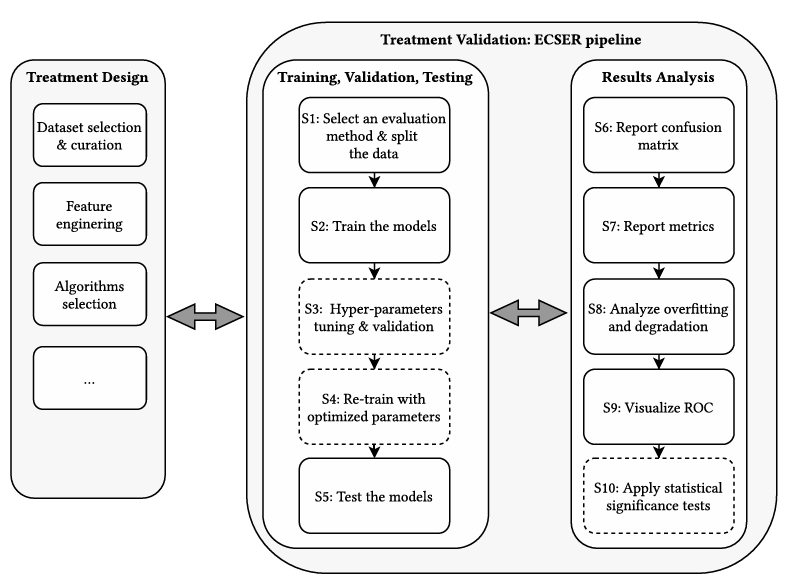
\includegraphics[width=0.8\linewidth]{figures/ECSER.png}
    \label{fig:ECSER}
\end{figure}


% What is the ECSER pipeline missing (LLMs) / Problems
However, while ECSER is tailored to traditional ML classifiers (such as logistic regression, SVMs and decision trees), it includes no specific recommendations for LLM-based classifiers, despite LLMs showing promise for various classification tasks \cite{Guo2024health,fields2024}. Thus, the ECSER pipeline is not sufficient for LLM research, since using LLMs for classification comes with unique considerations that are not present for traditional classifiers. For one, it is common to use pre-trained, generalized LLMs and give task-specific instructions to get the desired classification on the input data. This means that designing these instructions, also called prompts, becomes a crucial part to conducting LLM research \cite{Marvin2024}. There are also unique considerations when it comes to evaluating the fairness and robustness of the results: does the model behave in accordance with human values and are the results resilient to adversarial prompts, such as those containing typos \cite{Woodworth2017,zhu2024}?



% Contributions that will be made
The goal of this thesis is to address the lack of LLM-specific guidelines in the ECSER pipeline, by expanding it to include specific recommendations for conducting LLM classifier research. In doing so, we will make the following contributions:
\begin{itemize}
    \item We will conduct a mapping study to assess the current state of reporting in LLM4SE classification research.
    \item We will develop an expanded version of the ECSER pipeline that includes specific recommendations for conducting LLM classifier research, such as prompt engineering and the evaluation of model fairness and robustness.
    \item We will conduct two replication studies of existing LLM classifier papers using the enhanced pipeline, in order to evaluate the pipeline's usability and comprehensiveness.
\end{itemize}

% Structure of the thesis
The remainder of this thesis is structured as follows. In Section \ref{Background}, we provide background information about LLMs. Section \ref{Research approach} describes the research approach and research questions. Lastly, Section \ref{Related Work} discusses related work.

\section{Background}\label{Background}
% LLMs (what are LLMs, types of LLMs, prompt engineering)
\textbf{Language Models (LMs)} are computational models designed to model the generative likelihood of word sequences \cite{zhao2025}. In other words, given a sequence of input text, they predict the next word in the sequence based on what is deemed most likely by the model. One of the oldest examples of language models are N-grams, which model the likelihood of a word given the previous N tokens \cite{shannon1948}. Early statistical models like N-gram models suffer from several problems, including limited context and difficulty with unseen words.

\textbf{Pre-trained Language Models (PLMs)} are LMs that are designed to take in vast amounts of unannotated text in order to learn knowledge about language and the world \cite{jurafsky2025}. The knowledge that is contained in these models can then be used on new tasks by way of \textbf{transfer learning} \cite{wang2023plm}. PLMs require much more information to be contained within than statistical language models such as N-grams could provide, which has led researchers to design more sophisticated models that rely on neural networks to model language, starting with recurrent neural networks (RNNs) and later Long Short-Term Memory (LSTM) models \cite{mikolov2012rnn,hochreiter1997lstm}. The biggest recent breakthrough came with the invention of \textbf{transformers}, which performed better than previous models, were easier to train and allowed for the parallel processing of inputs \cite{Vaswani2017transformer}. Transformers typically consist of an \textbf{encoder}, which embeds the input sequence into a hidden (latent) space and a \textbf{decoder}, which translates the abstract representation of the hidden space to the target text. Both the encoder and decoder use a self-attention mechanism to weigh the contribution of each token to the output \cite{Vaswani2017transformer,bahdanau2016attention}.

\textbf{Large Language Models (LLMs)} were introduced as a way to refer to PLMs with massive parameter sizes, since it was found that larger parameter sizes lead to better performance and emergent abilities \cite{kaplan2020scaling,wei2022emergent}. Almost all LLMs use transformer models with the self-attention mechanism, but not all of them use both the encoder and decoder component \cite{hou2024}:
\begin{itemize}
    \item \textbf{Encoder-decoder LLMs}, such as BART \cite{lewis2019bart} and T5X \cite{roberts2022t5x}, are good at both understanding and generating language \cite{hou2024}. As such they are useful for tasks like summarization and translation \cite{cho2014encoderdecoder, Asadi2020encoderdecoder}.
    \item \textbf{Encoder-only LLMs}, such as BERT and its variants \cite{devlin2019bert,liu2019roberta,sanh2019distilbert,lan2020albert}, are tailored towards language understanding \cite{hou2024}. As such they are good at tasks like classification and inference \cite{koroteev2021encoder}. 
    \item \textbf{Decoder-only LLMs}, such as the GPT-series \cite{radford2018gpt,brown2020gpt3,openai2024gpt4}, are tailored towards language generation \cite{hou2024}. As such they are good at all generation tasks, including code generation \cite{poldrack2023} and creating conversational agents like ChatGPT \cite{OpenAI2023chatgpt} and LLama 2 \cite{touvron2023llama2}.
\end{itemize}




\textbf{Prompt Engineering} is the process of systematically designing natural language instructions (or \textbf{prompts}) to guide LLMs towards a desired output \cite{ronanki2023}. Prompts condition the outputs of the LLM on the given instructions, so that the model generates the next tokens with both the prompt and previously generated tokens in mind \cite{jurafsky2025}. The most common approaches to prompt engineering are:
\begin{itemize}
    \item \textbf{Zero-shot Prompting}. The model is given no examples for a task, forcing it to rely entirely on the prompt \cite{radford2019language}.
    \item \textbf{Few-shot Prompting}. A limited number of examples for a task are given, which the model can learn from \cite{brown2020fewshot}.
    \item \textbf{Chain-of-Thought Prompting}. The prompt instructs the model to follow coherent reasoning steps \cite{wei2022chain}.
\end{itemize}
Another less common approach is automatic prompt engineering, where instructions are automatically generated and selected \cite{zhou2023ape}.

\section{Research Approach} \label{Research approach}

% Research questions
The usage of LLMs in SE research has increased massively over the past few years, but the research of how to best conduct studies and report results in this field remains very limited. In order to approach the problem of LLM4SE reporting standards and design meaningful guidelines, we follow \citeauthor{Wieringa2014}'s design cycle of \textit{problem investigation}, \textit{treatment design} and \textit{treatment validation} \cite{Wieringa2014}. This leads us to the following research questions:

\emphasize{RQ1: What is the current state of reporting in LLM4SE classification research?} \\
% NOTE: Hou et al. and zhang et al. have very detailed search strategy and inclusion and exclusion criteria 
The purpose of RQ1 is both descriptive and evaluative: what do researchers report in their studies and does this level of reporting contribute or detract from the accuracy and reproducibility of the results. To answer the question, we conducted a mapping study of SE papers published in 2024 that use LLM classifiers using the guidelines by \citeauthor{kitchenham2011} \cite{kitchenham2011,kitchenham2007} and \textcite{petersen2008map}, consisting of five steps:
\begin{enumerate}
	\item Define the research question.
	\item Conduct a search for primary studies.
	\item Screen papers based on inclusion/exclusion criteria.
	\item Classify the papers.
	\item Extract data. 
\end{enumerate}
 What follows is a detailed summary of the search strategy (steps 2 and 3) and the information that was obtained from the list of relevant papers (steps 4 and 5). 

\textbf{Search Strategy}\\
To get a complete image of the state of LLM4SE classifier evaluation, we collected all 528 papers published in 2024 in three of the top SE conferences and journals (table \ref{table:venues}). These venues were narrowed down from the list of venues included in \cite{hou2024} based on their impact and relevance. Using the full list of 528 papers, an automatic keyword search was conducted on the title and abstract of each paper to identify the papers that were potentially relevant to LLM4SE.

The list of keywords was based on previous research (\cite{zhang2024,hou2024}) and designed with the intent of high recall, since it is easier to remove false positives than to retrieve false negatives. Keyword matching was done on the lowercased versions of the title and abstract and allowed for partial matches (e.g., "llm" matches "LLM", "LLMs", "LLM4SE", etc.). The complete list of keywords is as follows:
\begin{itemize}
	\item \textit{llm, large language model, language model, code generation model, plm, pre-trained, pretrained, pre-training, pretraining, chatgpt, gpt, bert, t5, llama, bart.}
\end{itemize}

The keyword search resulted in 129 potentially relevant papers. After manually removing false positives, mostly caused by the authors comparing their non-LLM model to previous LLM models, the total number of identified LLM4SE papers was 116, representing 21.97\% of total SE papers. 

To narrow down the list from all LLM-related papers to those pertaining to SE classification research, the title and abstract of the remaining 116 papers were manually screened for the inclusion and exclusion criteria (table \ref{table:criteria}). While only classification papers were included in the final mapping study, all the papers that applied LLMs to SE tasks (a total of 83 papers) were additionally classified based on the type of LLM application (classification, generation or recommendation) to get a view of the relative academic interest in each application type (figure \ref{fig:LLMTypes}). After applying all inclusion and exclusion criteria, 18 papers were identified that use LLMs for SE classification research and satisfy all other criteria.

\begin{table}[H]
    \raggedright
    \caption{Publication venues included in the mapping study.}
    \begin{tabularx}{\textwidth}{|c|X|} \hline
        \textbf{Acronym} & \textbf{Venue} \\ \hline
        ICSE  & International Conference on Software Engineering \\ \hline
        FSE   & International Conference on the Foundations of Software Engineering \\ \hline
        TSE   & Transactions on Software Engineering \\ \hline
    \end{tabularx}
    \label{table:venues}
\end{table}

\begin{table}[H]
    \caption{Inclusion/Exclusion Criteria}
    \begin{tabularx}{\textwidth}{|X|} \hline
        \textbf{Inclusion Criteria} \\ \hline
        The paper uses an LLM.  \\
        The paper focuses on a downstream application of the LLM. \\
        The downstream application is a SE classification task. \\
        The full text of the paper is accessible. \\
        The paper was published in 2024. \\ \hline
        \textbf{Exclusion Criteria} \\ \hline
        The paper focuses on LLM architecture with no downstream application. \\
        The paper or task is not relevant to SE. \\
        The full text is inaccessible. \\
        The paper is a survey or other meta-analysis. \\
        The paper focuses on research methodology. \\
        The paper is a reprint or different version of another paper. \\ \hline
    \end{tabularx}
    
    \label{table:criteria}
\end{table}

\begin{figure}
	\caption{Distribution of LLM applications in collected studies.}
	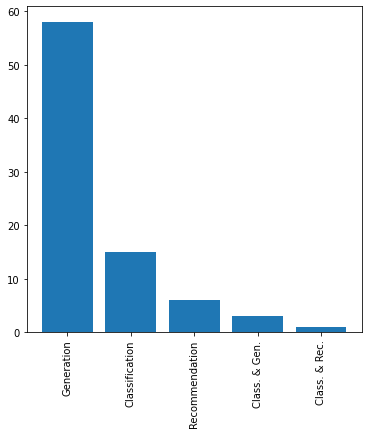
\includegraphics[width=0.6\linewidth]{figures/LLMTypes.png}
	\label{fig:LLMTypes}
\end{figure}

The information that was extracted from the papers was (BE EXACT) be determined based on what is recommended to be included by the ECSER pipeline \cite{Dellanna2022}, metrics that are recommended by other authors (such as the Matthews correlation coefficient \cite{Chicco2020,Foody2023,Yao2020}) and metrics and other information relevant to LLMs, like prompting technique and measures of fairness \& robustness (see section \ref{Prompt Engineering} and \ref{Evaluation of LLM Classifiers}). 

\emphasize{RQ2: What resource can be developed to assist researchers in conducting and reporting on LLM4SE classification research?}\\
RQ2 takes the role of treatment design; how can we solve potential problems that are identified by RQ1? The purpose of RQ2 is to design an artifact that is easy to use and comprehensive. To answer the question, we will enhance the existing ECSER pipeline \cite{Dellanna2022} to include the use of LLMs, taking into consideration recommendations from the fields of LLM4SE and ML4SE, as well as relevant statistical or methodological research in other fields (see section \ref{Related Work}). Table \ref{table:additions} includes a preliminary summary of the additions that will be made to the ECSER pipeline, with the primary supporting references for the additions in brackets. The list of additions is subject to change based on the findings from RQ1 and further literature review. It is also possible that the best course of action will be to add more steps to the ECSER pipeline, as opposed to expanding existing ones, particularly for reporting the calibration, fairness and robustness or for prompt engineering.

\begin{table}[H]
    \centering
    \caption{Preliminary summary of additions to the ECSER pipeline}
    \begin{tabularx}{\textwidth}{|p{4cm}|X|}
    \hline
    \textbf{ECSER Step} & \textbf{Additions} \\ \hline
    S1. Select an evaluation method and split the data             & Analyse desired level of model alignment and safety \cite{guo2023survey} \\ \hline
    \multirow[c]{3}{=}{S2. Train the model}                        & Define the goal of the prompt \cite{Marvin2024,arvidsson2023} \\ 
                                                                   & Select prompt engineering approach (zero-shot, few-shot, etc.)  \cite{hou2024,arvidsson2023} \\ 
                                                                   & Select prompting pattern \cite{white2023,arvidsson2023} \\ \hline
    \multirow[c]{2}{=}{S3. Hyper-parameters tuning and validation} & Tune LLM model temperature \cite{peeperkorn2024} \\ 
                                                                   & Compare prompting patterns \cite{ronanki2023} \\ \hline
    \multirow[c]{4}{=}{S7. Report Metrics}                         & Report Matthews correlation coefficient (MCC) \cite{Chicco2020,Foody2023,Yao2020} \\ 
                                                                   & Report calibration (e.g., expected calibration error \cite{Pakdaman2015}) \\ 
                                                                   & Report fairness (e.g., equalized odds difference \cite{Woodworth2017}) \\ 
                                                                   & Report robustness (e.g., performance drop rate \cite{zhu2024}) \\ \hline
    \end{tabularx}
    
    \label{table:additions}
\end{table}


\emphasize{RQ3: How useful is the proposed pipeline in assisting LLM4SE classification research?}\\
The purpose of RQ3 is treatment validation: does the designed pipeline in RQ2 achieve its goals of ease of use and comprehensiveness. To answer this question we will conduct two replication studies in different subfields of SE that employ LLM classification using the guidelines by \textcite{carver2010}. The original studies will be chosen based on the following criteria:
\begin{enumerate}
    \item The authors provide a ready-to-use replication package.
    \item The study is recent (past five years) and represents current practices in LLM4SE well.
    \item The study is peer-reviewed and published in a reputable journal.
    \item The study does not already follow all the proposed guidelines, so that the added benefit of the pipeline can be evaluated.
\end{enumerate}

By conducting these replication studies, we can evaluate the comprehensiveness of the pipeline and identify potential shortcomings. In order to test the ease of use for the intended users, we aim to ask an SE researcher to use the pipeline or give their expert opinion on it if possible. After the first replication study, the findings from RQ3 will be taken into account to make changes to the guidelines from RQ2 where needed, creating a feedback-loop between RQ2 and RQ3. The second replication will be conducted using the updated pipeline and might inform further changes.

\textbf{Timeline}\\
The below table proposes a timeline for each step of the research project. It is subject to change if certain parts take more or less time than expected.
\begin{table}[ht]
\caption{Timeline}
\begin{tabular}{|l|l|}
\hline
\textbf{Period} & \textbf{Activity} \\ \hline
Week 21–24 & RQ1: Conduct and analyse mapping study \\ \hline
Week 25–26 & RQ2: Design enhanced ECSER pipeline \\ \hline
Week 27–35 & Summer break \\ \hline
Week 36–39 & RQ2: Design enhanced ECSER pipeline (contd.) \\ \hline
Week 40–45 & RQ3: Conduct and analyse replication studies \\ \hline
Week 46–48 & Finish thesis \\ \hline
Week 49–50 & Prepare and hold thesis defence \\ \hline
\end{tabular}
\end{table}

\section{Related Work} \label{Related Work}
The main focus of this thesis is to study the usage and evaluation of LLM Classifiers in Software Engineering, but in doing so we touch on several related research fields, including Empirical Software Engineering, Machine Learning for Software Engineering (ML4SE), Large Language Models for Software Engineering (LLM4SE) and Prompt Engineering. Additionally, each of the three research questions has related work that is relevant to their methodologies. Hence, we have split the related work into several sections based on different areas of study to aid readability. 

First, we discuss challenges in empirical software engineering which motivated the creation of the ECSER pipeline and further motivate our mapping study of LLM4SE. Second, we discuss the topic of replication in SE, which is relevant to our replication studies and the field of empirical SE. Third, we discuss how Large Language Models have been used in SE, with a focus on classification tasks. Fourth, we discuss related work in Prompt Engineering, as it has become a vital part to using LLMs and will inform our guidelines for prompt engineering in the enhanced ECSER pipeline. Finally, we discuss related work on the evaluation of LLMs and classifiers which will inform our guidelines for the evaluation of LLM Classifiers.

\subsection{Challenges in Empirical Software Engineering}
% Related work on evaluating "simple" classifiers in SE (Dell'ana 2022, Kitchenham 2004, Kitchenhham 2002, Menzies 2012, Zhang 2002)
Over the past couple decades, the use of machine learning methods has become ubiquitous in every field of science, among them software engineering. \textcite{Zhang2002} summarized seven main activities that use machine learning in SE: prediction, property/model discovery, transformation, generation, library construction and maintenance, acquisition of specifications and development knowledge management. In addition, they list specific tasks belonging to each activity, such as \textit{predicting} software quality and \textit{generating} test cases. The field of classification research falls almost exclusively in the prediction category.

With the increased popularity of machine learning methods, many software packages have been developed to allow anyone to use these methods without having to write any code or even understand how these methods work. This leads to many researchers using machine learning without fully understanding the underlying assumptions of the methods they are using and assuming the results are correct without proper (statistical) analysis. This problem is not new: \textcite{kitchenham2002} reported at the start of this century that there was a poor standard of empirical software engineering, mostly caused by a lack of statistical expertise from both the authors and reviewers. They go on to provide extensive guidelines for designing and conducting experiments as well as analysing, presenting and interpreting results. In another paper, \textcite{kitchenham2004} discuss the benefits of evidence-based software engineering approach by drawing an analogy to evidence-based medicine, but note that the infrastructure needed for widespread adoption of evidence-based SE isn't there yet, which means that SE experiments are vulnerable to subject and experimenter bias. 

Methodological problems in SE research can result in problems with the reproducibility of results, which severely reduces the real-world usefulness of said results. \textcite{Menzies2012} argue that the main goal of science is \textit{conclusion stability}, which means that when you discover an effect, it holds true irrespective of the situation. However, they note that in the software engineering literature there is often as much evidence \textit{for} a given effect, as \textit{against}. This lack of conclusion stability is caused by sources of bias and variance that are introduced at various steps: sampling, pre-processing, training, algorithm selection and the analysis of results. If these sources of bias and variance are accurately analysed and reported, that would make it easier for the authors and other researchers to interpret the conclusions.

Despite being a known issue, the problems of improper analysis and reporting have persisted over the years. In a mapping study of the proceedings of the International Conference of Software Engineering (ICSE) from 2019 to 2021, \textcite{Dellanna2022} analysed 60 SE papers related to classification and found that most papers (36) reported on the precision and recall of their experiment, fewer reported the F-score (27) and accuracy (24), but only 14 papers explicitly justified why they chose the reported metrics. The full confusion matrix was only included in six papers. Other metrics like the receiver operator characteristic (ROC) curve and the area under the curve (AUC) were mostly absent with 3 and 9 respective mentions. Of course, as we know from statistics, it is not enough to report a metric and claim it's better than that of other models, since it could be coincidental, so statistical significance testing is required to make such claims. However, only six papers analysed the statistical significance of their results. Evidently, the situation is dire, which is why \citeauthor{Dellanna2022} developed the ECSER pipeline to give SE researchers a systematic approach to conducting classification experiments and reporting and analysing the results. 

\subsection{Replications in SE}
Replication studies are a vital part of empirical software engineering, allowing researchers to investigate the effects of alternative values for important attributes, vary the strategy with which hypotheses are investigated and make up for certain threats to validity \cite{Basili1999}. The importance of replication is not unique to software engineering, after all the so-called "replication crisis" was a massive topic of debate in psychology research in recent years, since it was found that many previous results in the field could not be replicated, even if the original findings were statistically significant \cite{Shrout2018,Maxwell2015,Amrhein2018}. \textcite{Cruz2020} conducted a systematic literature review of replication studies in SE between 2013 and 2018 and found that the number of published replication studies has been steadily increasing, though there are research gaps in certain fields, suggesting that the SE community is taking an increased interest in replicating previous studies.

\textcite{Shull2008} identify two types of replication studies: \textit{exact replications}, in which the procedures of the original study are strictly followed; and \textit{conceptual replications}, in which the research problem of the original study is evaluated using a different procedure. Additionally, exact replications are subdivided into \textit{dependent} and \textit{independent} replications. Dependent replications keep most of the conditions of the experiment (close to) the same, which allows one to test the effect of specific variables on the results; whereas independent replications vary the original conditions of the experiment significantly, which allows one to test the robustness of the original results under different conditions. \textcite{Juristo2010} underline the value of non-exact replications, which they define similarly to how \citeauthor*{Shull2008} define independent exact replications, by conducting a multiple-case replication study using a newly proposed four-phase process, to show that non-identical replications can be used to learn new information about the original results.

While there is a consensus in SE that replication is important, \textcite{Shepperd2018} show that replication studies often suffer from the same problems as original studies, such as incomplete reporting, low power or potential researcher bias. Notably, many replication studies in their survey did not report any details on the dispersion (e.g., variance) of the response variables. In another paper, \textcite{Shepperd2018b} shows that because of wide prediction intervals, almost all replications are confirmatory, which means the added knowledge is negligible. Because of these problems, they suggest that researchers should focus more on broader meta-analyses instead of replication studies. Other common problems in conducting replication research include difficulty in getting them published, lack of guidelines and the unavailability of replication packages \cite{Cruz2020,Siegmund2015}.

Communication can also play a factor in successful replication: \textcite{Vegas2006} investigated the role of communication in successful replication of previous experiments and found that there should be some level of communication, orally or in writing, between the previous authors and authors of the replication study, to avoid unnecessary changes to the experiments. 

Given these challenges, guidelines for conducting replications are clearly needed. Despite this, the number of existing guidelines remains low. Guidelines were proposed by \textcite{carver2010}, which are still commonly used in replications, but these seem to be the only replication guidelines for software engineering and were intended as a starting point for future guidelines. Other artifacts do exist to aid replications: \textcite{Gomez2014} proposed a classification of replications in SE, differentiating between literal, operational and conceptual replications, that can be used to identify which changes can be made in each type of replication and understand the level or verification needed for that type. 

\textcite{Abualhaija2024} proposed an artifact, referred to as the ID-Card, for summarizing papers in RE research that use NLP techniques. The intention behind the ID-Card is that all the relevant information needed for replication is presented in an easy to read format and can be used for both replication and educational purposes. Lastly, \textcite{Brandt2014} developed the "Replication Recipe" for psychology research, which lists 36 questions that should be addressed when conducting a replication, most of which are also directly applicable to empirical SE. 

\subsection{Large Language Models for SE}
% Related work on LLMs in SE in general (Wang 2024, Fan 2023, find more for specific subdomains?)
A recent development in SE research is the increased relevance and use of LLMs. \textcite{fan2023} looked at all preprints on arXiv categorised under computer science whose title included "LLM", "Large Language Model" or "GPT" and found the number of SE papers that mentioned LLMs grew exponentially from 0 in 2019, 5 in 2020, to 181 in 2023. Naturally, this is only an approximation of the total number of preprints on arXiv that use LLMs, but it undoubtedly signifies a substantial increase. \citeauthor{fan2023} also conducted an extensive survey of how LLMs have been applied to various software development activities (such as code generation and testing) and research domains (such as human-computer interaction and education), but the survey is almost exclusively focused on the generative use of LLMs and does not go into depth on the use of LLMs in classification research. Many other good surveys and analyses of the use of LLMs in Software Engineering have been written, but most of them similarly do not mention any applications to classification tasks and instead exclusively focus on generation \cite{Belzner2024,Zheng2024,Ozkaya2023}.

Surveys have also been written about specific domains of software engineering: \textcite{wang2024} did a comprehensive review of 102 studies that use LLMs for software testing and found that LLMs have commonly been applied to various tasks, including test case generation, test input generation, debugging, program repair and more\comment{REWRITE WITH TABLE OF TASKS}. They also found that while most papers used LLMs to address the entire task, many others combined LLMs with additional techniques to optimize the outputs of the LLM, including mutation testing, differential testing, syntactic checking, program analysis, statistical analysis and other techniques. With these extra techniques, researchers were able to generate more diverse and complex code and overcome some of the limitations of LLMs. 

% Related work on LLMs in CLASSIFICATION (Hou 2024, Zhang 2024, Fields 2024)
While LLMs are most frequently used to generate text (and code), they have seen considerable success in classification tasks. \textcite{Guo2024health} have shown that LLMs can outperform other methods like SVMs for health-related text classification. \textcite{fields2024} present an in-depth survey of text classification using transformers across domains and found that LLMs can perform remarkably well on many (but not all) classification tasks. However, \textcite{Chen2024} compared the performance of various LLMs to traditional ML methods in clinical prediction and found that LLMs could \textit{not} beat traditional methods in this case. \textcite{vajjala2025} also show that there are large performance disparities between languages in classification tasks. Thus, LLMs might not always be a better choice than traditional ML methods, but they certainly show potential. 

Software engineers have also started using LLMs for classification. \textcite{hou2024} conducted a systematic literature review of 395 software engineering studies that use LLMs and found that around 21.61\% involve classification tasks. The most common classification tasks where LLMs have been used include vulnerability detection, requirements classification, bug prediction and review/commit/code classification, with many other classification tasks having been attempted using LLMs. \textcite{zhang2024} conducted a systematic survey of 947 SE studies and summarized 62 unique LLMs of code, including six LLMs specifically fine-tuned for the tasks of code classification, clone detection and defect detection.


\subsection{Prompt Engineering} \label{Prompt Engineering}
% Prompt engineering (Hou 2024, Arvidsson 2023, Ronanki 2023, Ekin 2023, White 2023, Marvin 2024)
Designing a good prompt for a particular task is vital to ensuring the adequate performance of LLMs, which is why much research has gone into the systematic designing of prompts, or prompt engineering. \textcite{Marvin2024} provide an overview of prompt engineering principles and techniques and outline the main steps involved in the process of prompt engineering: 1) define the goal of the prompt; 2) understand the model's capabilities; 3) choose the right prompting format; 4) provide context to the LLM and 5) test and refine the prompt based on the goal. Several resources exist to make it easier to choose the right prompting approach: \textcite{white2023} introduce prompt patterns, which offer reusable solutions to common prompting challenges, and provide a framework for designing and documenting these patterns in terms of the intent, motivation, structure and consequences of the patterns. For example, the persona pattern can be used to make the LLM take the point of view of an expert in the field, which is especially useful if the user itself is not an expert. The paper provides a catalogue of this pattern and other successfully applied patterns with example implementations. Further, \textcite{ekin2023} provides an accessible (AI-generated) guide to prompt engineering.

Prompt engineering research has also been conducted specifically for software engineering: \textcite{hou2024} looked at what prompt engineering techniques are commonly applied in SE tasks and found the most common techniques involve few-shot prompting and zero-shot prompting, but the third largest group of studies had no explicit mention of prompting techniques or proposed their own strategies. Other techniques included chain-of-thought, automatic prompt engineering, chain-of-code, automatic chain-of-thought, modular-of-thought and structured chain-of-thought.

\textcite{arvidsson2023} collected prompt engineering recommendations for requirements engineering (RE) in a systematic literature review and classified the guidelines into various themes, after which they interviewed three RE experts to evaluate the guidelines. \textcite{ronanki2023} evaluated the effectiveness of 5 prompting patterns (from the catalogue by \textcite{white2023}) on two RE tasks and proposed a framework for evaluating the effectiveness of prompting patterns for any RE task, providing five steps for conducting a comparison of patterns.

A recent development in prompt engineering is automatic prompt engineering (APE), which has shown good performance compared to baseline models, while avoiding the need for manually designing prompts \cite{zhou2023ape,ye2024ape}. \textcite{zadenoori2025} investigated the use of automatic prompt engineering in RE and found that, on average, APE outperforms traditional prompt engineering techniques. However, research is still limited.

\subsection{Evaluating LLM Classifiers} \label{Evaluation of LLM Classifiers}
% Evaluation of classifiers (ECSER, papers mentioned in ECSER)
Few papers have been written specifically about the evaluation of LLM-based classifiers, but we can look at the evaluation of classifiers and LLMs separately to get a picture. The ECSER pipeline is the most relevant for evaluating classifiers, since it gives in-depth recommendations about the conducting and reporting of classifier research \cite{Dellanna2022}. Specific recommendations include the reporting of the full confusion matrix, reporting other metrics relevant to the domain such as specificity (true negative rate), analysing overfitting and degradation, visualising the ROC and applying statistical significance tests. Some researchers also recommend reporting the Matthews correlation coefficient (MCC), which combines all four metrics of the confusion matrix and can be more informative than the F1 score \cite{Chicco2020,Foody2023,Yao2020}. 

\textcite{hou2024} looked at whether these metrics were reported in LLM-based classification research and found that out of 147 papers that use LLMs for classification, the most frequently reported metric is precision with 35 papers, followed by recall (34), F1-score (33) and accuracy (23), but the AUC was reported 9 times, the ROC only 4 times and the MCC only twice. Unfortunately, they did not count how many studies did significance testing. These results are very similar to \textcite{Dellanna2022}'s aforementioned mapping study of classifier research as a whole and suggest that many important metrics are under-reported in LLM-based classification research. 

% Evaluation of LLMs/LLM classifiers (guo 2023, chang 2023) 
Using and evaluation LLMs comes with more considerations than just the accuracy of the results. \textcite{guo2023survey} categorize the evaluation of LLMs into three types: knowledge and capability evaluation, which assesses the fundamental knowledge and reasoning capabilities of the LLM; alignment evaluation, which refers to evaluating ethical and moral considerations like bias; and safety evaluation, which focuses on the robustness of LLMs and risk evaluation. \textcite{liu2024} have created guidelines specifically for evaluating LLM alignment in terms of reliability, safety, fairness, resistance to misuse, explainability and reasoning, adherence to social norms and robustness. 

Another consideration is how well the LLM outputs adhere to the format specified in the prompt. For example, it is common to ask an LLM to format its answer as a valid JSON object, allowing for easier processing of the output. Limiting responses to a specified format can be beneficial: \textcite{tam2024format} compared the performance of several LLMs between free-form response and formatted responses and found that, while reasoning ability was weakened for formatted responses, classification accuracy was increased. However, LLMs do not always follow the format accurately. \textcite{long2025format} define several measures to analyse the level of adherence to the output format: SysE, which measures the performance of the LLM for answers that \textit{meet the constraint}; TrueE, which measures the performance of all answers \textit{regardless of whether the format is satisfied}; and BiasF, which measures the (mean squared) difference between SysE and TrueE. \textcite{Li2024format} introduce the JScore measure, which measures the similarity between JSON objects and can be used to compare LLM generated JSON objects with the target JSON objects. Lastly, \textcite{xia2024fofo} introduce the FoFo benchmark for evaluating LLMs based on their ability to follow complex, domain-specific formats. 

\textcite{chang2023} conducted another survey of the evaluation of LLMs which focuses on downstream applications, resulting in a classification of four aspects of LLM evaluation: the accuracy, containing measures of correctness such as the F1 score; the calibration, which contains measures for the degree of alignment between the predicted probabilities and actual probabilities, such as the expected calibration error (ECE); the fairness, with measures pertaining to the equal treatment of different groups, such as the equalized odds difference (EOD); and robustness, with measures pertaining to the performance of a model in the face of challenging inputs and noise, such as performance drop rate (PDR). Further, they mention several ways in which human evaluation can be used to evaluate LLMs, such as the degree to which the model outputs align with human values.

Lastly, the model temperature, which regulates the randomness of the model, can also affect its performance. \textcite{peeperkorn2024} looked at the effect of model temperature on the level of creativity of the outputs and found that LLMs generate slightly more novel outputs with higher temperature, but the temperature was also correlated with incoherence. No relationship was found between temperature and cohesion or typicality. Model temperature might also affect a model's susceptibility to security attacks: \textcite{Yu2024} found that some LLMs became more susceptible to jailbreaking attacks as temperature increased, whereas others had decreased susceptibility to jailbreaking with increased temperature, possibly due to the fact that the former models had a lower susceptibility at 0 temperature and the latter models had a higher susceptibility at 0 temperature.

\newpage
\printbibliography[heading=bibintoc]

\begin{appendices}
\section{Additional Mapping Study Results}
For brevity, sources were excluded for some figures and are included here for further reference. 
\begin{table}[ht]
	\caption{Classification of LLM application types.}
	\begin{tabularx}{\textwidth}{|l|c|X|}
	    \hline
	    \textbf{Category} & \textbf{Number of studies} & \textbf{References} \\ \hline
		Generation & 58 & [To be filled] \\ \hline
		Classification & 15 & [To be filled] \\ \hline
		Recommendation & 6 & [To be filled] \\ \hline
		Generation \& Classification & 3 & [To be filled] \\ \hline
		Classification \& Recommendation & 1 & [To be filled] \\ \hline
	\end{tabularx}
\end{table}
\end{appendices}

\end{document}
